\documentclass[12pt,a4paper]{article}

% \newcommand*{\TypeChinese}{} % Chinese support
\newcommand*{\AdvancedDocument}{} % include code and math
\newcommand*{\WithHeader}{}

% basic packages
\usepackage[margin=2cm]{geometry}
\usepackage{graphicx,subfigure,indentfirst,hyperref,colortbl,caption,cite,color,xcolor,tikz,}
\hypersetup{colorlinks=true,urlcolor=blue,linkcolor=blue}

\ifdefined\AdvancedDocument
	% minted is better than listing.
	\usepackage{minted}
	% it requires minted of a newer version.
	\setminted{linenos=true, frame=lines, framesep=2mm}	
	\usepackage{amsmath,amssymb,bm}
\fi

\ifdefined\TypeChinese
	\usepackage{xeCJK,fontspec}
	\XeTeXlinebreaklocale "zh"
	\XeTeXlinebreakskip = 0pt plus 1pt
	\setmainfont{KaiGen Gothic TW}
	\setCJKmainfont{KaiGen Gothic TW}
	\setmonofont{Droid Sans Mono}
	\renewcommand{\baselinestretch}{1.3}
\fi

\ifdefined\WithHeader
	\usepackage{fancyhdr}
	\fancypagestyle{plain}{
		\fancyhf{}
		\chead{GPU Programming 2016 Spring \textbar ~CSIE Department, National Taiwan University}
		\cfoot{\thepage}
		\rfoot{GPGPU Assignment \#1 Hint}
	}
	\pagestyle{plain}
	\renewcommand{\headrulewidth}{1pt}
	\renewcommand{\footrulewidth}{2pt}
\fi

\newcommand{\figref}[1]{Figure \ref{Fig:#1}.}
\newcommand{\tabref}[1]{Table \ref{Tab:#1}.}
\newcommand{\lstref}[1]{Listing \ref{Lst:#1}.}
% \graphicspath{{fig/}}

\begin{document}

Have you heard the "binary indexed tree"?

\begin{itemize}
\item \url{https://leetcode.com/problems/range-sum-query-mutable/}
\item \url{http://www.csie.ntnu.edu.tw/~u91029/Sequence.html#8}
\end{itemize}

\vspace{3cm}
More hints in the next page $\downarrow$.

\pagebreak

\begin{figure}[H]
\centering
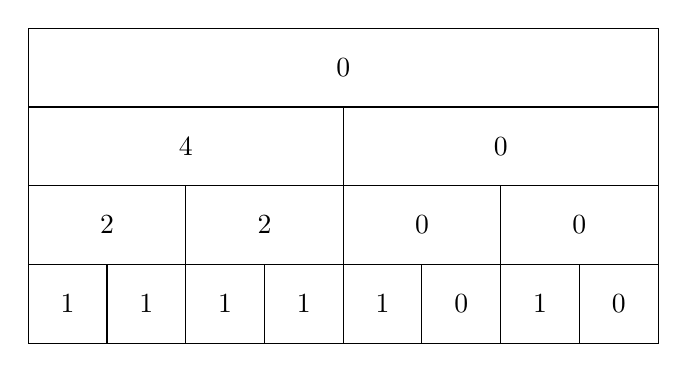
\begin{tikzpicture}[scale=1]
\draw (0,0) rectangle (8,4);
\foreach \y in {1,...,3}
	\draw (0,\y) -- (8,\y);
\foreach \h/\n/\start in {1/4/1,2/2/2,3/1/4} {
	\foreach \x in {1,...,4} {
		\draw (\start*\x*2-\start,0) -- (\start*\x*2-\start,\h);	
		\ifnum \x=\n
			\breakforeach
		\fi
	}
}
\node at (0.5,0.5) {1};
\node at (1.5,0.5) {1};
\node at (2.5,0.5) {1};
\node at (3.5,0.5) {1};
\node at (4.5,0.5) {1};
\node at (5.5,0.5) {0};
\node at (6.5,0.5) {1};
\node at (7.5,0.5) {0};

\node at (1,1.5) {2};
\node at (3,1.5) {2};
\node at (5,1.5) {0};
\node at (7,1.5) {0};

\node at (2,2.5) {4};
\node at (6,2.5) {0};

\node at (4,3.5) {0};
\end{tikzpicture}
\caption{The binary indexed tree}
\end{figure}

The upper level is:
\begin{itemize}
\item Addition of the lower 2 levels if they are both non-zero.
\item 0, otherwise.
\end{itemize}

\vspace{3cm}
More hints in the next page $\downarrow$.

\pagebreak

\begin{figure}[H]
\centering
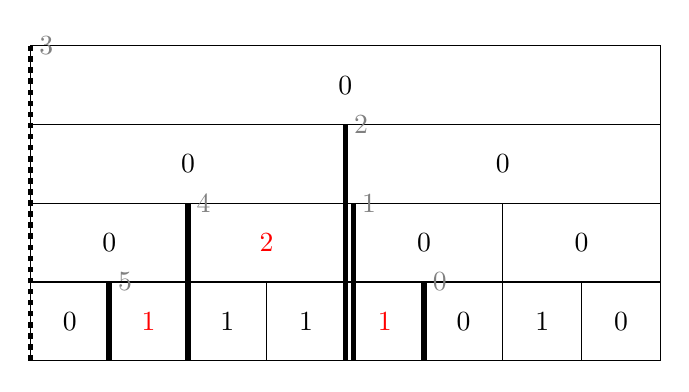
\begin{tikzpicture}[scale=1]
\draw (0,0) rectangle (8,4);
\foreach \y in {1,...,3}
	\draw (0,\y) -- (8,\y);
\foreach \h/\n/\start in {1/4/1,2/2/2,3/1/4} {
	\foreach \x in {1,...,4} {
		\draw (\start*\x*2-\start,0) -- (\start*\x*2-\start,\h);
		\ifnum \x=\n
			\breakforeach
		\fi
	}
}
\node at (0.5,0.5) {0};
\node at (1.5,0.5) {\textcolor{red}{1}};
\node at (2.5,0.5) {1};
\node at (3.5,0.5) {1};
\node at (4.5,0.5) {\textcolor{red}{1}};
\node at (5.5,0.5) {0};
\node at (6.5,0.5) {1};
\node at (7.5,0.5) {0};

\node at (1,1.5) {0};
\node at (3,1.5) {\textcolor{red}{2}};
\node at (5,1.5) {0};
\node at (7,1.5) {0};

\node at (2,2.5) {0};
\node at (6,2.5) {0};

\node at (4,3.5) {0};
\draw[line width=2pt] (5,0) -- (5,1); \node at (5.2,1) {\textcolor{gray}{0}};
\draw[line width=2pt] (4.1,0) -- (4.1,2); \node at (4.3,2) {\textcolor{gray}{1}};
\draw[line width=2pt] (4,0) -- (4,3); \node at (4.2,3) {\textcolor{gray}{2}};
\draw[line width=2pt,dotted] (0,0) -- (0,4); \node at (0.2,4) {\textcolor{gray}{3}};
\draw[line width=2pt] (2,0) -- (2,2); \node at (2.2,2) {\textcolor{gray}{4}};
\draw[line width=2pt] (1,0) -- (1,1); \node at (1.2,1) {\textcolor{gray}{5}};
\end{tikzpicture}
\caption{The binary indexed tree}
\end{figure}

\begin{table}[H]
\centering
\begin{tabular}{llll}
\hline
\hline
Check & Result & Length & Loop invariant \\
\hline
Try to add 1 to align to 2 & OK      & 1 & Align to 2 \\
Try to add 2 to align to 4 & Already & 1 & Align to 4 \\
Try to add 4 to align to 8 & Fail    & 1 & Align to 4, less than 4 more 1's\\
Try to add 2               & OK      & 3 & Less than 2 more 1's\\
Try to add 1               & OK      & 4 & Less than 1 more 1's (done)\\
\hline
\hline
\end{tabular}
\caption{The Algorithm}
\end{table}

We traverse the tree bottom-up then top-down.
This algorithm can handle at most $(2^h-1)$ 1's
where $h$ is the height of the tree.
So you have to choose $h = 9$ to handle $k = 500$.

Note that we also illustrate the "OK", "Already" and initial state by bold black lines while "Fail" is dotted bold lines.

\vspace{3cm}

One more example in the next page $\downarrow$.
\pagebreak

\begin{figure}[H]
\centering
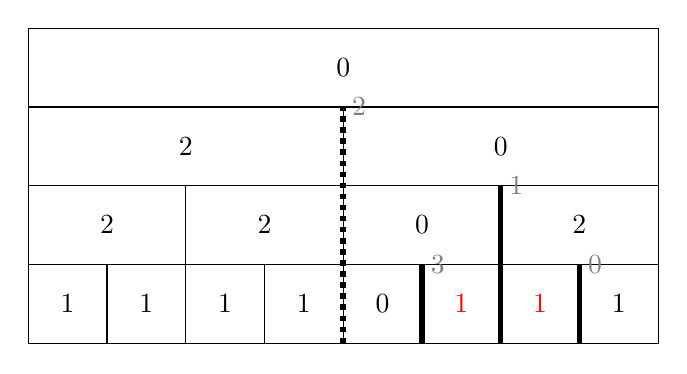
\begin{tikzpicture}[scale=1]
\draw (0,0) rectangle (8,4);
\foreach \y in {1,...,3}
	\draw (0,\y) -- (8,\y);
\foreach \h/\n/\start in {1/4/1,2/2/2,3/1/4} {
	\foreach \x in {1,...,4} {
		\draw (\start*\x*2-\start,0) -- (\start*\x*2-\start,\h);
		\ifnum \x=\n
			\breakforeach
		\fi
	}
}
\node at (0.5,0.5) {1};
\node at (1.5,0.5) {1};
\node at (2.5,0.5) {1};
\node at (3.5,0.5) {1};
\node at (4.5,0.5) {0};
\node at (5.5,0.5) {\textcolor{red}{1}};
\node at (6.5,0.5) {\textcolor{red}{1}};
\node at (7.5,0.5) {1};

\node at (1,1.5) {2};
\node at (3,1.5) {2};
\node at (5,1.5) {0};
\node at (7,1.5) {2};

\node at (2,2.5) {2};
\node at (6,2.5) {0};

\node at (4,3.5) {0};
\draw[line width=2pt] (7,0) -- (7,1); \node at (7.2,1) {\textcolor{gray}{0}};
\draw[line width=2pt] (6,0) -- (6,2); \node at (6.2,2) {\textcolor{gray}{1}};
\draw[line width=2pt] (5,0) -- (5,1); \node at (5.2,1) {\textcolor{gray}{3}};
\draw[line width=2pt, dotted] (4,0) -- (4,3); \node at (4.2,3) {\textcolor{gray}{2}};
\end{tikzpicture}
\caption{The binary indexed tree}
\end{figure}

\begin{table}[H]
\centering
\begin{tabular}{llll}
\hline
\hline
Check & Result & Length & Loop invariant \\
\hline
Try to add 1 to align to 2 & OK      & 1 & Align to 2 \\
Try to add 2 to align to 4 & Fail    & 1 & Align to 2, less than 2 more 1's\\
Try to add 1               & OK      & 2 & Less than 1 more 1's (done)\\
\hline
\hline
\end{tabular}
\caption{The Algorithm}
\end{table}

In this example we "Fail" at the lower level.

\vspace{3cm}
Sadly I have no more hint for you.

\end{document}
